\documentclass[11pt,english]{article}

\usepackage[english]{babel}
\usepackage{enumitem}
\usepackage{fancyhdr}
\usepackage[top=2.3cm, bottom=2.3cm, left=1.6cm, right=1.6cm]{geometry}
\usepackage{graphicx}
\usepackage{lastpage}
\usepackage{tabularx}
\usepackage{listings}
\usepackage{color}
\usepackage{eurosym}

\definecolor{dkgreen}{rgb}{0,0.6,0}
\definecolor{gray}{rgb}{0.5,0.5,0.5}
\definecolor{mauve}{rgb}{0.58,0,0.82}

\lstset{frame=tb,
	language=SQL,
	aboveskip=3mm,
	belowskip=3mm,
	showstringspaces=false,
	columns=flexible,
	basicstyle={\small\ttfamily},
	numbers=none,
	numberstyle=\tiny\color{gray},
	keywordstyle=\color{blue},
	commentstyle=\color{dkgreen},
	stringstyle=\color{mauve},
	breaklines=true,
	breakatwhitespace=true,
	tabsize=3
}

\pagestyle{fancy}
\setlength{\parindent}{0pt}        % indentation on new paragraph
\setlength{\parskip}{0pt}          % vertical spacing on new paragraph
\setlength{\lineskip}{1pt}         % vertical spacing between lines
\setlength{\columnsep}{1cm}        % spacing between columns
\setlength{\belowcaptionskip}{0pt} % spacing below captions
\setlength{\abovecaptionskip}{5pt} % spacong above captions

\graphicspath{{assets/}}

\lfoot{}
\cfoot{\today}
\rfoot{\thepage/\pageref{LastPage}}

\newcommand*{\Frontpage}{\begingroup
	\hbox{%
		\hspace*{0.2\textwidth}
		\rule{1pt}{\textheight}
		\hspace*{0.05\textwidth}
		\parbox[b]{0.75\textwidth}{%
			{\noindent\Huge\bfseries DATAB3}\\[2\baselineskip] % Title
			{\large \textit{Huiswerkopdrachten, week 6}}\\[4\baselineskip] % Tagline or further description
			{\Large \textsc{\\
				Patrick Spek, 2099745 \\
				Chris Meesters, 2098474 \\
			}}
			\vspace{0.5\textheight} % Whitespace between the title block and the publisher
		}
	}
\endgroup}

\renewcommand{\footrulewidth}{0.4pt}

\begin{document}
	\thispagestyle{empty}
	\Frontpage

	\newpage
	\tableofcontents

	\newpage
	\section{Hoelang staan de leningen open?}
	\subsection{Schermafdrukken}
	\subsubsection{Gesorteerd op aantal dagen}
	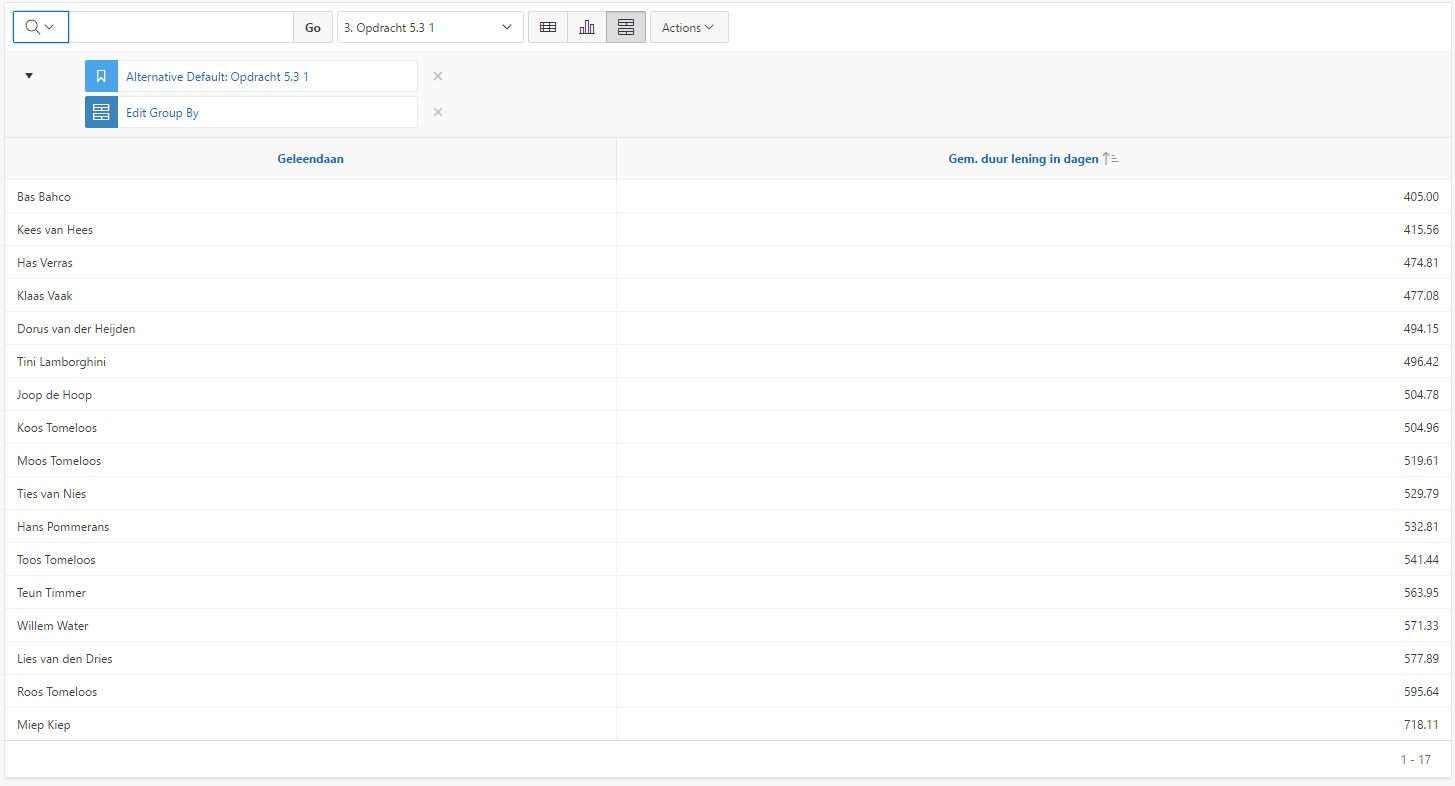
\includegraphics[scale=0.5]{week6-openstaande-leningen}

	\subsubsection{Als staafdiagram}
	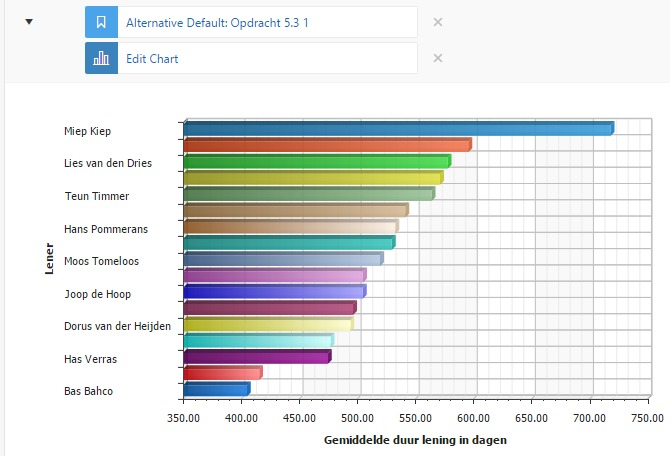
\includegraphics[scale=0.5]{week6-openstaande-leningen-staafdiagram}

	\subsection{SQL queries}
	\begin{lstlisting}
SELECT ps.Voornaam, ROUND(AVG(ln.Datumterugbetaald - ln.Datumgeleend)) gem_duur FROM lening ln
JOIN persoon ps ON ln.NUMMER = ps.NUMMER 
GROUP BY ps.Voornaam
ORDER BY gem_duur ASC
	\end{lstlisting}

	\newpage
	\section{In welke maand wordt het meeste geleend?}
	\subsection{Schermafdukken}
	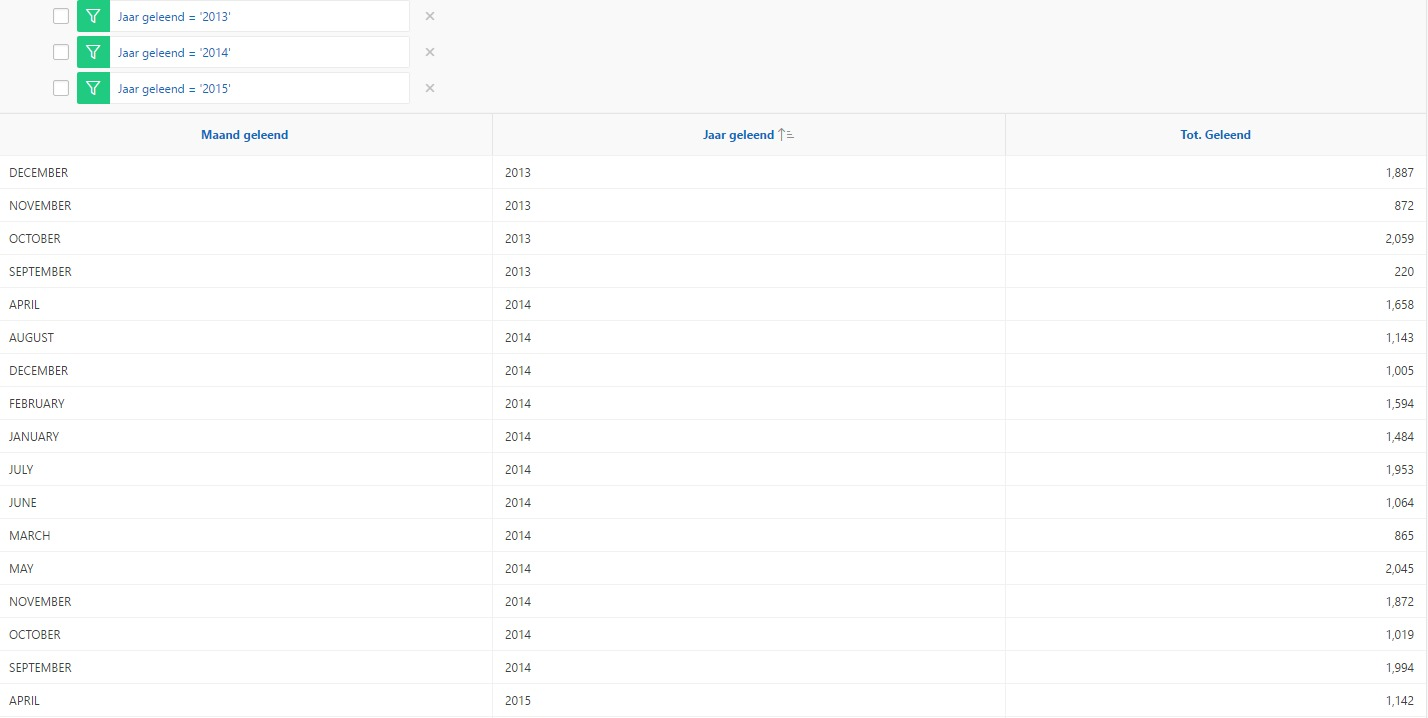
\includegraphics[scale=0.5]{week6-overzicht}

	\subsection{SQL queries}
	\subsubsection{Aangepaste view definitie}
	\begin{lstlisting}
CREATE OR REPLACE VIEW "LENING_INFO"
	("BEDRAG", "DATUMGELEEND", "DATUMTERUGBETAALD", "STATUS", "GELEENDVAN", "GELEENDAAN", "RENTE", "BEDRAG_MET_RENTE", "MAAND_GELEEND", "JAAR_GELEEND") AS
SELECT
	lng.bedrag,
	lng.datumgeleend,
	lng.datumterugbetaald,
	decode(lng.terugbetaald,'Y','Terugbetaald','Niet terugbetaald') status,
	p_van.voornaam|| ' ' ||p_van.achternaam geleendvan,
	p_aan.voornaam|| ' ' ||p_aan.achternaam geleendaan,
	lng.rente,
	bereken_rente(lng.bedrag,lng.rente,lng.datumgeleend) bedrag_met_rente,
	to_char(lng.datumgeleend, 'MONTH') as maand_geleend,
	to_char(lng.datumgeleend, 'YYYY') as jaar_geleend
FROM
	lening lng
JOIN
	persoon p_aan on lng.geleendaan = p_aan.nummer
JOIN
	persoon p_van on lng.geleendvan = p_van.nummer
	\end{lstlisting}

	\newpage
	\section{Applicatiegegevens}
	\begin{tabular}{ l l }
		\textbf{URL} & https://apex.oracle.com/pls/apex/f?p=110443:1:3614339805312::::: \\
		\textbf{Domain} & \texttt{DATBAS3} \\
		\textbf{User} & \texttt{JOKIP7@GMAIL.COM} \\
		\textbf{Password} & \texttt{Ab12345} \\
	\end{tabular}
\end{document}

